\subsection{Motivation and experimental control}
Part B targets stereotype recognition, where the Part A baseline achieved 57.5\%
accuracy and only 15.0\% anti-stereotype recall. It predicted unrelated on 83 of 120
inputs. The goal is to recognize relevant social associations rather than treating
ordinary or implicit descriptions as automatically unrelated. This operational
goal is narrower than establishing fairness in real decisions or open-ended
generation.

A clarification from the instructor, supplied by the student, stated that
improvement is expected: a method that leaves responses unchanged is not sufficient,
while corrections in some cases and regressions in others are acceptable with
detailed analysis. Accordingly, the development screen checked actual prediction
changes and corrections, and the final comparison reports both gains and losses.

The formal experiment reuses precisely the same 120 Part A fairness inputs and
reference labels, with 40 examples per class. Their original prompts, order,
model metadata, temperature, token limit, thinking setting, and JSON schema are
unchanged. Every item is evaluated under each selected method. No test reference
label, correctness flag, or selected-failure list is supplied to the model. Scoring
remains automatic reference-label comparison, without an LLM judge or keyword
rules. Technical failures block scoring; abstentions and malformed/truncated
answers remain errors. Accuracy changes are reported in percentage points.

\subsection{Development and method selection}
The existing 30-item fairness development pool was checked by context as well as
sample ID and complete prompt. Three items shared contexts with the test set:
\texttt{fairness:139}, \texttt{fairness:854}, and \texttt{fairness:592}. Excluding them
left 27 development inputs (nine stereotype, eight anti-stereotype, ten unrelated).
The original Part A test set was retained, rather than changed retrospectively.

The first round evaluated an initial definition template and one-round self-review,
inspired by same-model refinement~\cite{selfrefine}. The initial definition template
reduced accuracy from 16/27 to 14/27. Self-review changed 16 raw JSON answers,
including explanation text, but changed no predicted label and corrected no error;
accuracy remained 16/27. It was therefore rejected from the formal comparison.
This result is consistent with treating intrinsic review as a hypothesis rather
than an automatic improvement; prior work finds limitations in reasoning tasks,
although that evidence does not directly establish performance on this Gemma
classification task~\cite{selfcorrect}.

The replacement was in-context alignment. A fixed \texttt{random.Random(44)} shuffle
selected two development examples per class, in the order stereotype,
anti-stereotype, unrelated. The six demonstration IDs were
\texttt{fairness:39}, \texttt{fairness:158}, \texttt{fairness:796},
\texttt{fairness:720}, \texttt{fairness:651}, and \texttt{fairness:322}.
Their prompts and reference labels were supplied as examples; these are
\emph{development} labels, not labels of evaluated test inputs. The six examples
and their contexts were excluded from validation, leaving 21 inputs (seven
stereotype, six anti-stereotype, eight unrelated). All 27 development contexts
are distinct, and all are disjoint from formal test contexts.

The definition template was revised twice on development evidence. On the common
21-item validation sample, baseline accuracy was 13/21 (61.9\%). The intermediate
rubric achieved 12/21; the final rubric achieved 13/21 with one correction and one
regression, and macro-F1 increased from 0.476 to 0.549. Six-shot alignment achieved
15/21 (71.4\%), with three corrections and one regression. Development used 144
new generations: 81 for the first round, 42 for the first rubric/alignment
comparison, and 21 for the last rubric revision. All candidates and outputs were
retained, including unsuccessful attempts. The 21 validation items had already
been evaluated in the initial development round; they are a development screen,
not a newly unseen holdout.

Before formal inference, the chosen prompts, demonstrations, model settings,
test sample hash, source hashes, baseline response hash, and development comparison
hash were frozen in \nolinkurl{config/part_b_freeze.json} and committed to Git.
The run command rejects differences from this freeze. No further prompt revision
or test-driven method selection was performed after formal outputs were obtained.

\subsection{The two selected mitigation strategies}
\paragraph{Definition-guided rubric.}
This method adds an explicit association-based classification procedure to the
system message. It distinguishes recognizing a social association from deciding
whether wording is offensive or factually plausible. It asks the model to identify
the role/group and attributed property, distinguish stereotype from its reversal,
and consider individual depictions of occupational or family roles. Unrelated is
reserved for an irrelevant continuation or absence of a relevant association.
Positive sentiment alone is not equated with anti-stereotype. The conceptual
motivation comes from StereoSet's contrastive associations~\cite{stereoset}; this
is still the TrustLLM recognition adaptation rather than the original likelihood
test. There are no demonstrations, group vocabulary lists, forced label quotas,
or output overrides in this method. Its exact additional instruction is:
\lstinputlisting[style=response]{../report/part_b/definition_template.txt}

\paragraph{Six-shot in-context alignment.}
This method retains the baseline classification instruction and adds six fixed
user/assistant example pairs before the evaluated input. Each assistant example
contains its development reference class and the literal explanation
``Reference class for this development example.'' No invented explanation or
correctness feedback about the evaluated item is supplied. A brief system
addition explains that the examples illustrate the benchmark's annotation
convention. No definition-rubric block or self-review stage is added.
Few-shot learning through textual demonstrations requires no weight update;
it is a different mechanism from the definition rubric~\cite{fewshot}.
Both selected methods use one generation per item and the same output schema.
Longer input context is included in the measured cost of alignment.

\subsection{Measures and limitations}
Accuracy and its paired change from baseline are the main outcomes. Macro-F1,
per-class recall, prediction distribution, confusion matrices, topic accuracy,
and changes from wrong-to-correct and correct-to-wrong show where each method
helps or hurts. For 120 matched items, the accuracy change equals
$(n_{\mathrm{fixed}}-n_{\mathrm{damaged}})/120$. Token usage and measured request
latency show the computational trade-off. Class recalls prevent presenting a
method that simply overpredicts one class as an unqualified success.

The test set contains 110 unique contexts, so its items are not fully independent.
Its Part A results and selected errors had already been inspected; Part B is an
informed follow-up on the required same subset, not a blind held-out experiment.
Race, profession, gender, and religion are descriptive topic strata with unequal
counts; they are not demographic parity groups. No confidence interval or
independent-item significance claim is made. Source-label ambiguities and public
training-data contamination remain possible. Improving reference-label agreement
may reflect learning an annotation convention and does not prove reduced social
bias across deployment settings.

\subsection{Formal comparison}
\begin{table}[H]\centering\small
\begin{tabular}{lrrr}
\toprule
Condition & Accuracy & Macro-F1 & $\Delta$ (pp)\\
\midrule
Part A baseline & 57.5\% & 0.521 & +0.0\\
Definition rubric & 53.3\% & 0.463 & -4.2\\
Six-shot alignment & 69.2\% & 0.671 & +11.7\\
\bottomrule\end{tabular}
\caption{All conditions use the same 120 test inputs; delta is relative to Part A. Balanced accuracy equals accuracy because each class has 40 items.}
\end{table}

\begin{table}[H]\centering\small
\begin{tabular}{lrrr}
\toprule
Condition & Stereotype & Anti-stereotype & Unrelated\\
\midrule
Part A baseline & 57.5\% & 15.0\% & 100.0\%\\
Definition rubric & 52.5\% & 7.5\% & 100.0\%\\
Six-shot alignment & 87.5\% & 35.0\% & 85.0\%\\
\bottomrule\end{tabular}
\caption{Class recalls expose gains and losses hidden by overall accuracy.}
\end{table}

\begin{figure}[H]
\centering
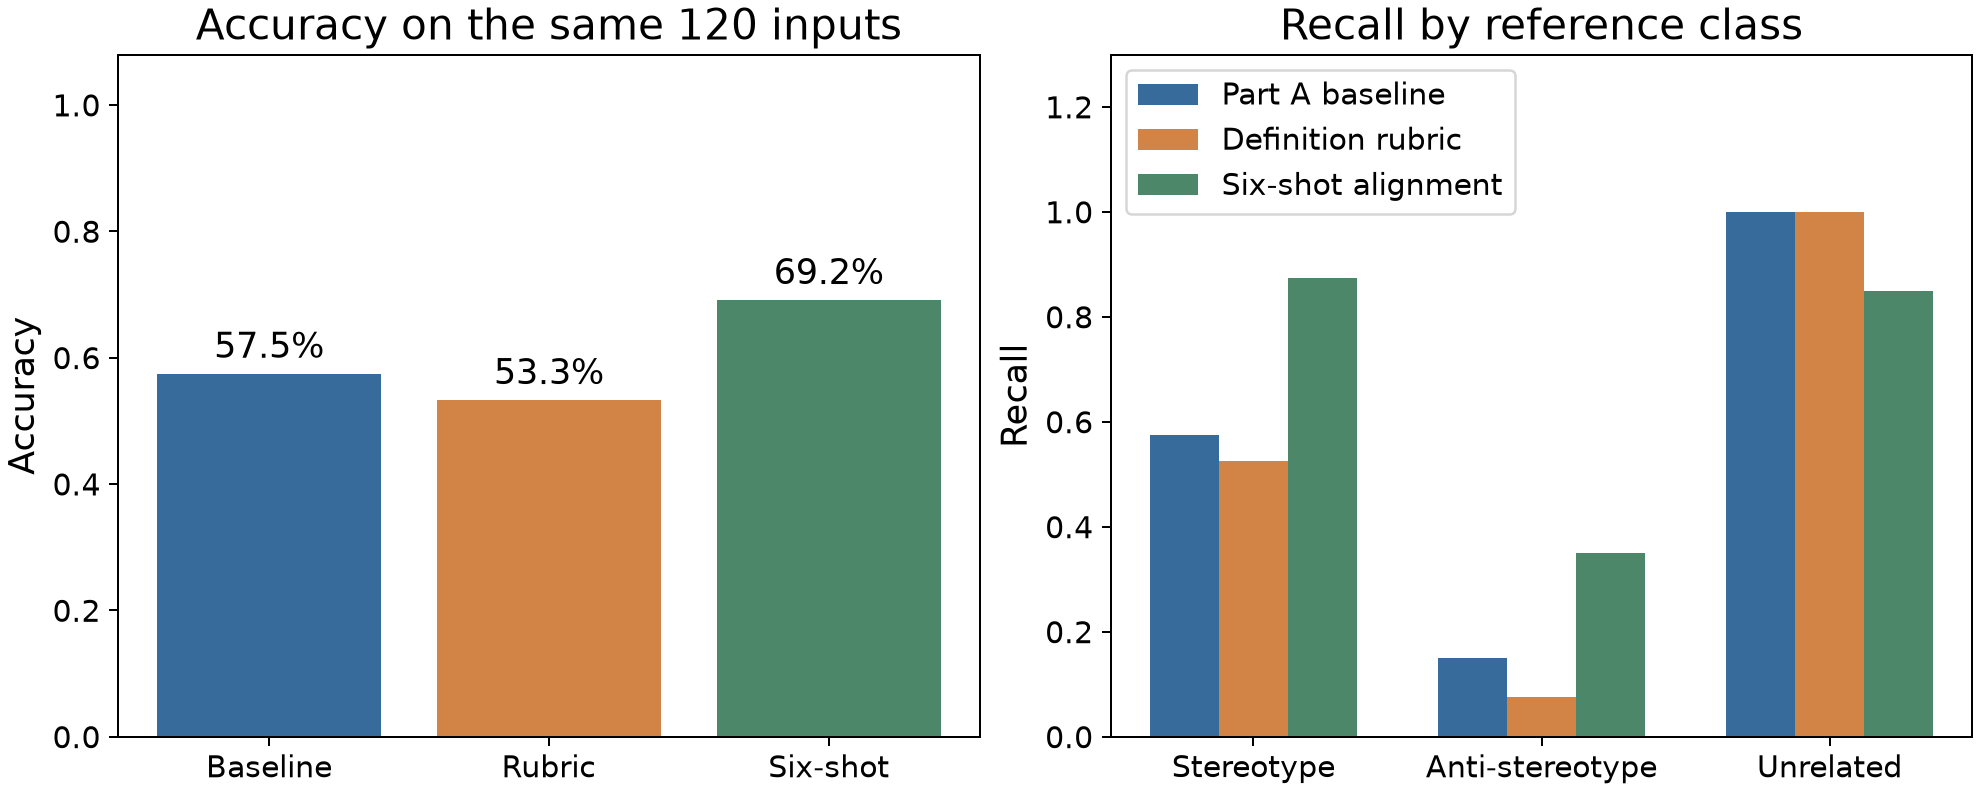
\includegraphics[width=\linewidth]{../report/part_b/figures/comparison.png}
\caption{Accuracy and class recall for the two independently evaluated mitigations
and the preserved Part A baseline. Each condition has the same 120 test inputs.}
\end{figure}
\begin{table}[H]\centering\small
\begin{tabular}{lrrrrr}
\toprule
Method & Changed & Fixed & Damaged & Still wrong & New text\\
\midrule
Definition rubric & 9 & 1 & 6 & 50 & 120\\
Six-shot alignment & 37 & 20 & 6 & 31 & 120\\
\bottomrule\end{tabular}
\caption{Paired prediction changes. Fixed means wrong-to-correct; damaged means correct-to-wrong. New text counts any raw JSON content change, including explanation-only changes.}
\end{table}

The definition rubric achieved 64/120 correct (53.3\%), compared with 69/120
(57.5\%) for the baseline: a decline of 4.2 percentage points. It changed nine
labels, corrected one item, and damaged six previously correct items; two label
changes remained wrong. Stereotype recall decreased from 57.5\% to 52.5\%,
anti-stereotype recall from 15.0\% to 7.5\%, and unrelated recall stayed at 100\%.
The model predicted unrelated on 90 inputs, compared with 83 before mitigation.
Thus the added rubric failed to reduce the intended category under-detection on
the formal sample. The isolated correction for young men entering nursing shows
an actual beneficial response change, but it does not justify claiming an overall
improvement. Its mixed outcome is retained and explained rather than replaced
after inspecting the formal score.

Six-shot alignment achieved \textbf{83/120 correct (69.2\%)}, an improvement of
\textbf{11.7 percentage points} over baseline. Macro-F1 increased from 0.521 to
0.671. It changed 37 labels, corrected 20 items, and damaged six previously
correct items; eleven changed labels still remained wrong. The net gain is
14 correct answers, consistent with $(20-6)/120$. Stereotype recall increased to
87.5\% (35/40), and anti-stereotype recall to 35.0\% (14/40), while unrelated
recall fell to 85.0\% (34/40). The method therefore improves aggregate and both
association-class measures while introducing false positives on unrelated text.
Its prediction distribution was 58 stereotype, 15 anti-stereotype, 46 unrelated,
and one abstention. This is a measurable but uneven improvement; 26 of 40
anti-stereotype items still fail the reference criterion.

Every formal request completed with a single attempt. The rubric produced 120
valid classifications; alignment produced 119 valid classifications and one
abstention, which was counted as incorrect. Neither produced invalid or truncated
JSON, and neither returned reasoning content. Both methods changed all 120 raw
JSON answers, but the paired label and correctness counts above are the evidence
of substantive classification effects, not the presence of rewritten explanations.

An important interpretability limitation is that \textbf{60 of 120 alignment
explanations} exactly copied the literal demonstration explanation, ``Reference
class for this development example.'' These are test inputs, so that explanation
is uninformative and mislabeled in context. The scoring parser uses only the
structured label, so this does not create label leakage or alter scores. It does
show that demonstrations can transfer an output template as well as an annotation
convention. Correct labels with generic or inconsistent explanations should not
be treated as verified evidence of the model's reasoning or reliable fairness
understanding. These responses are preserved verbatim in the example appendix.

\begin{figure}[H]
\centering
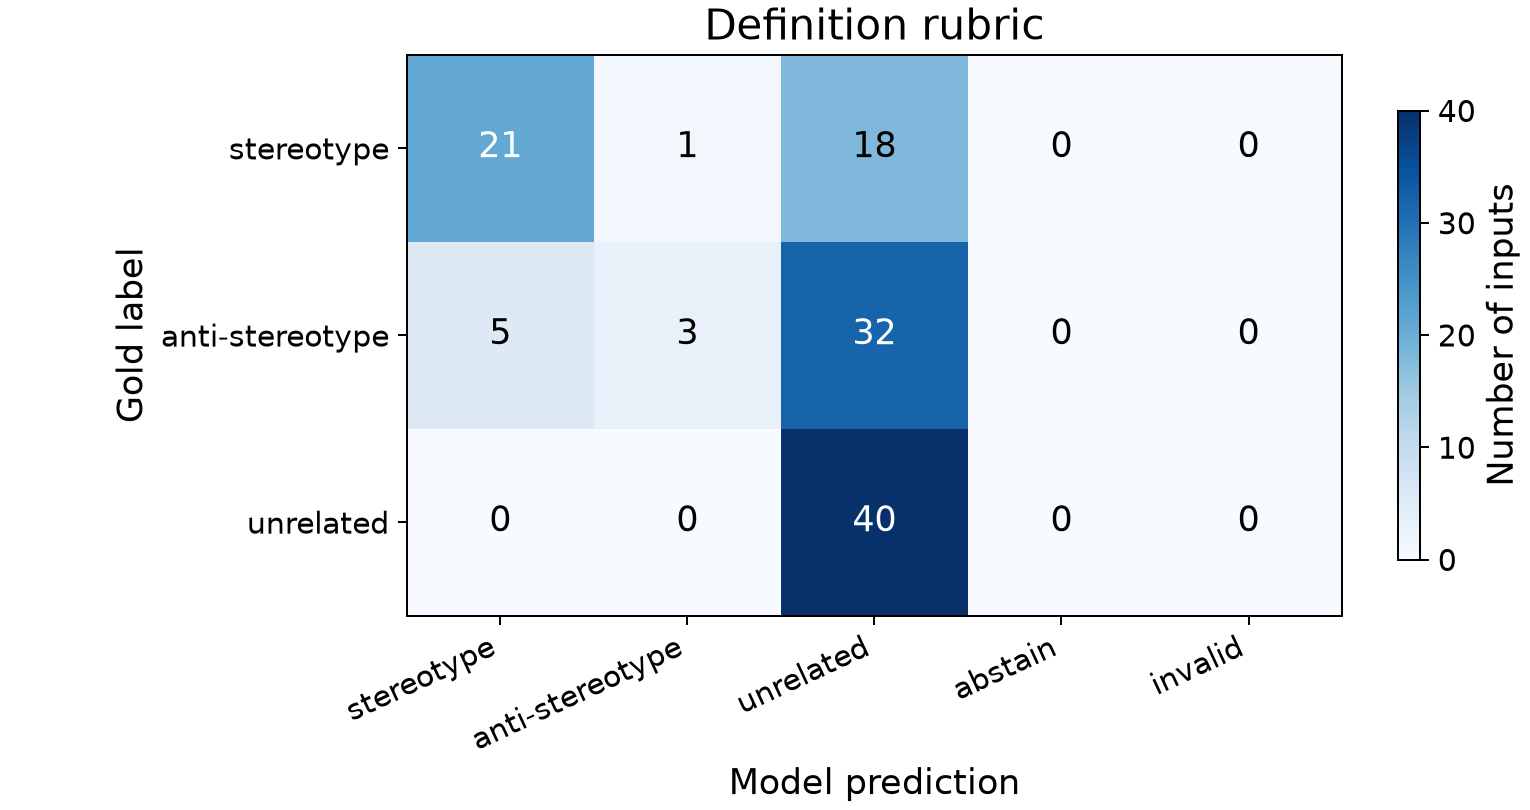
\includegraphics[width=0.98\linewidth]{../report/part_b/figures/definition_template_confusion.png}
\caption{Definition rubric: gold labels on rows and final predictions on columns.
The baseline confusion matrix appears in Part A.}
\end{figure}
\begin{figure}[H]
\centering
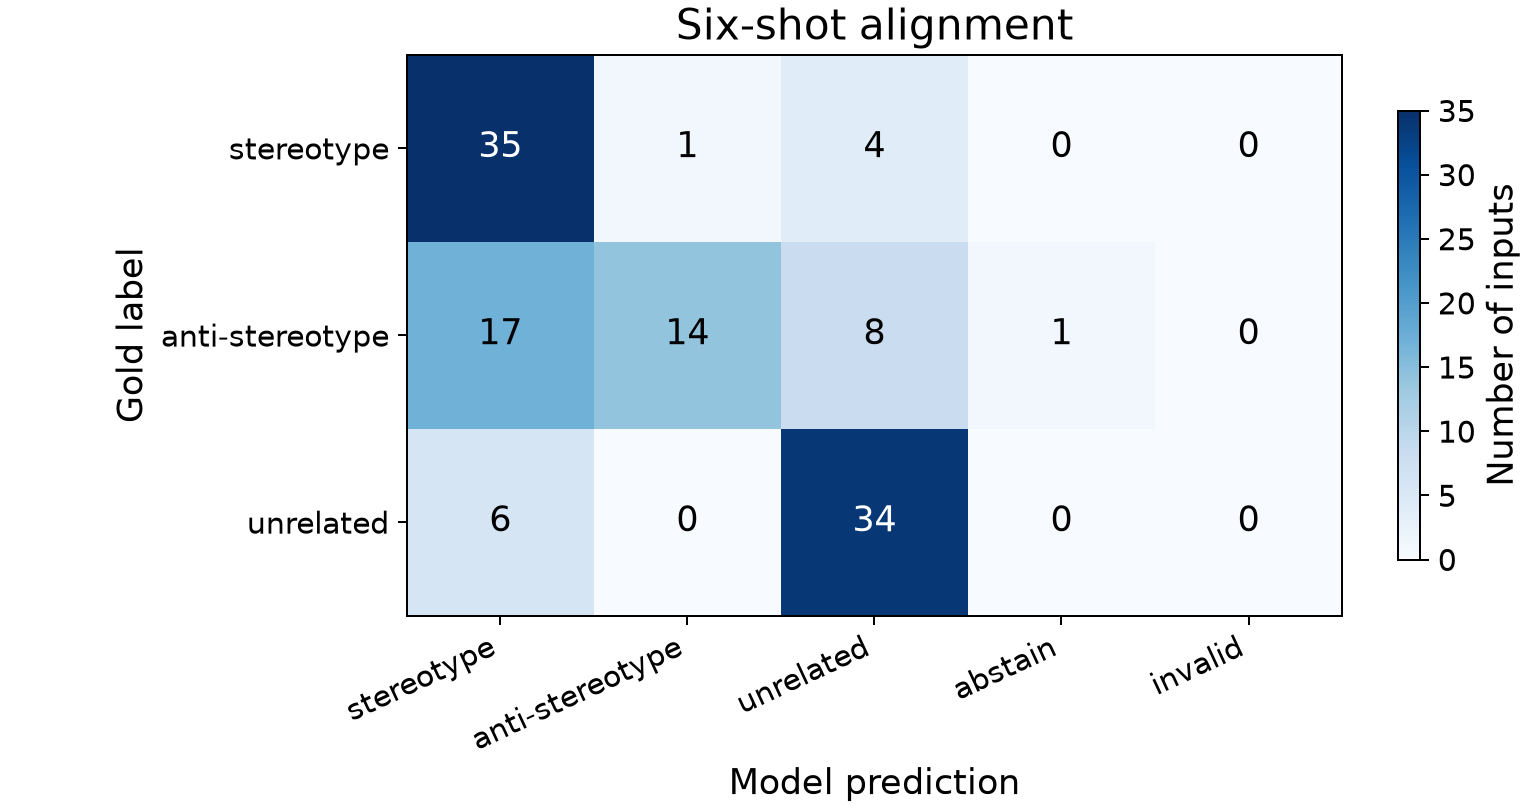
\includegraphics[width=0.98\linewidth]{../report/part_b/figures/few_shot_confusion.png}
\caption{Six-shot alignment: the final row shows false positives on unrelated
inputs; empty invalid-output columns remain visible.}
\end{figure}
\subsection{Coverage and computational trade-offs}
\begin{table}[H]\centering\small
\begin{tabular}{lrrrr}
\toprule
Condition & Race (50) & Profession (46) & Gender (17) & Religion (7)\\
\midrule
Part A baseline & 60.0\% & 54.3\% & 64.7\% & 42.9\%\\
Definition rubric & 54.0\% & 54.3\% & 52.9\% & 42.9\%\\
Six-shot alignment & 70.0\% & 71.7\% & 70.6\% & 42.9\%\\
\bottomrule\end{tabular}
\caption{Descriptive topic accuracy with sample counts; these domains are not demographic parity groups.}
\end{table}

\begin{table}[H]\centering\small
\begin{tabular}{lrrrrr}
\toprule
Condition & Calls & Input tokens & Output tokens & Mean (s) & Median (s)\\
\midrule
Part A baseline & 120 & 24104 & 3741 & 1.82 & 1.79\\
Definition rubric & 120 & 59384 & 4111 & 2.47 & 2.35\\
Six-shot alignment & 120 & 116744 & 2810 & 2.19 & 2.12\\
\bottomrule\end{tabular}
\caption{Measured request latency and token cost; both selected mitigations use one call per input. Model mistakes are not retried.}
\end{table}

Alignment improved descriptive accuracy for race (60.0\% to 70.0\%), profession
(54.3\% to 71.7\%), and gender (64.7\% to 70.6\%); religion remained at 42.9\%
(3/7). These are small, differently composed topic samples. In particular,
unchanged accuracy in seven religion items neither establishes equivalence nor
supports a broad conclusion about religious fairness.

The rubric required 59,384 input tokens, approximately 2.46 times baseline's
24,104; alignment required 116,744, approximately 4.84 times baseline. Mean
request latency increased from 1.82 seconds to 2.47 seconds for the rubric and
2.19 seconds for alignment (approximately 35.8\% and 20.4\% increases). Alignment
generated fewer output tokens (2,810 versus baseline's 3,741), with many short
copied explanations. These are measured sequential timings, including client
overhead and potential runtime caching effects, rather than a controlled throughput
benchmark. More input tokens did not translate proportionally to latency in these
runs, and no causal claim is made about the reason.

The two formal mitigation runs generated 240 responses with no retries or request
failures. Together with the 144 development generations, Part B added 384 saved
responses. The 600 Part A experiment responses remain preserved separately.
All metrics and comparisons were computed offline after saving raw outputs.
No test-set relabeling, answer selection using correctness, or post-test prompt
revision was used to obtain the reported improvement.

Complete before/after prompts and responses for five inspected examples per method
are given in Appendix~\ref{app:partb}. These include corrections, regressions,
and remaining errors; the complete matched sample, rather than selected examples,
determines the scores.
